% Pengaturan ukuran teks dan bentuk halaman dua sisi
\documentclass[12pt]{book}

% Pengaturan ukuran halaman dan margin
\usepackage[a4paper,top=30mm,left=30mm,right=20mm,bottom=25mm]{geometry}

% Pengaturan ukuran spasi
\usepackage[singlespacing]{setspace}

% Pengaturan caption untuk tabel
\usepackage{caption}

% Judul dokumen
\title{Proposal Tugas Akhir ITS}
\author{Utomo, Satrio Heru} 

% Pengaturan detail pada file PDF
\usepackage[pdfauthor={\@author},bookmarksnumbered,pdfborder={0 0 0}]{hyperref}


% Pengaturan ukuran indentasi
\setlength{\parindent}{2em}

% Package lainnya
\usepackage{changepage}
\usepackage{etoolbox} % Mengubah fungsi default
\usepackage[section]{placeins}
% Pengaturan jenis karakter
\usepackage[utf8]{inputenc}

\usepackage[style=ieee, backend=biber]{biblatex}
\usepackage{enumitem} % Pembuatan list
\usepackage{lipsum} % Pembuatan template kalimat
\usepackage{graphicx} % Input gambar
\usepackage{longtable} % Pembuatan tabel
\usepackage[table,xcdraw]{xcolor} % Pewarnaan tabel
\usepackage{eso-pic} % Untuk menggunakan background image di halaman
\usepackage{txfonts} % Font times
\usepackage{changepage} % Pembuatan teks kolom
\usepackage{multicol} % Pembuatan kolom ganda
\usepackage{multirow} % Pembuatan baris ganda
\usepackage{tabularx} % Untuk mengatur kolom, seperti grid pada CSS
\usepackage{wrapfig}
\usepackage{float}
\usepackage[OT1]{fontenc} % Untuk mengatur jenis font dan encodingnya

% Pengaturan format daftar isi, daftar gambar, dan daftar tabel
\usepackage[titles]{tocloft}
\usepackage{subfig}
\setlength{\cftsecindent}{2em}
\setlength{\cftsubsecindent}{2em}
\setlength{\cftbeforechapskip}{1.5ex}
\setlength{\cftbeforesecskip}{1.5ex}
\setlength{\cftbeforetoctitleskip}{0cm}
\setlength{\cftbeforeloftitleskip}{0cm}
\setlength{\cftbeforelottitleskip}{0cm}
\renewcommand{\cfttoctitlefont}{\hfill\Large\bfseries} % command untuk membuat heading bold dan besar
\renewcommand{\cftaftertoctitle}{\hfill}
\renewcommand{\cftloftitlefont}{\hfill\Large\bfseries}
\renewcommand{\cftafterloftitle}{\hfill}
\renewcommand{\cftlottitlefont}{\hfill\Large\bfseries}
\renewcommand{\cftafterlottitle}{\hfill}

% Definisi untuk "Hati ini sengaja dikosongkan"
\patchcmd{\cleardoublepage}{\hbox{}}{
  \thispagestyle{empty}
  \vspace*{\fill}
  \begin{center}\textit{[Halaman ini sengaja dikosongkan]}\end{center}
  \vfill}{}{}

  % Pengaturan penomoran halaman
\usepackage{fancyhdr}
\fancyhf{}
\renewcommand{\headrulewidth}{0pt}
\pagestyle{fancy}
\fancyfoot[C,CO]{\thepage}
\patchcmd{\chapter}{plain}{fancy}{}{}
\patchcmd{\chapter}{empty}{plain}{}{}

% Command untuk bulan
\newcommand{\MONTH}{%
  \ifcase\the\month
  \or Januari% 1
  \or Februari% 2
  \or Maret% 3
  \or April% 4
  \or Mei% 5
  \or Juni% 6
  \or Juli% 7
  \or Agustus% 8
  \or September% 9
  \or Oktober% 10
  \or November% 11
  \or Desember% 12
  \fi}
\newcommand{\ENGMONTH}{%
  \ifcase\the\month
  \or January% 1
  \or February% 2
  \or March% 3
  \or April% 4
  \or May% 5
  \or June% 6
  \or July% 7
  \or August% 8
  \or September% 9
  \or October% 10
  \or November% 11
  \or December% 12
  \fi}

% Pengaturan format judul bab
\usepackage{titlesec}
\renewcommand{\thesection}{\thechapter.\arabic{section}}
\titleformat{\chapter}[hang]{\centering\bfseries\large}{BAB\ \arabic{chapter}\ }{0ex}{\vspace{0ex}\centering}
\titleformat*{\section}{\large\bfseries}
\titleformat*{\subsection}{\normalsize\bfseries}
\titlespacing{\chapter}{0ex}{0ex}{4ex}
\titlespacing{\section}{0ex}{1ex}{0ex}
\titlespacing{\subsection}{0ex}{0.5ex}{0ex}
\titlespacing{\subsubsection}{0ex}{0.5ex}{0ex}
\setcounter{secnumdepth}{3} % Untuk memberi penomoran pada \subsubsection

\counterwithin{figure}{chapter}
\counterwithin{table}{chapter}

% Mengganti figure dan table menjadi gambar dan tabel
\renewcommand{\figurename}{Gambar}
\renewcommand{\tablename}{Tabel}

% Atur variabel berikut sesuai namanya

% nama
\newcommand{\name}{Satrio Heru Utomo}
\newcommand{\authorname}{Utomo, Satrio Heru}
\newcommand{\nickname}{Satrio}
\newcommand{\advisor}{Dr. Supeno Mardi Susiki Nugroho, ST., MT.}
\newcommand{\coadvisor}{Reza Fuad Rachmadi, S.T., M.T., Ph.D}
\newcommand{\examinerone}{Dosen, S.T., M.T.}
\newcommand{\examinertwo}{Dosen, S.T., M.Sc.}
\newcommand{\examinerthree}{Dosen, S.T., M.T.}
\newcommand{\headofdepartment}{Prof. Dosen, S.T., M.T}

% identitas
\newcommand{\nrp}{0721 19 4000 0053}
\newcommand{\advisornip}{19700313 199512 1 001}
\newcommand{\coadvisornip}{19850403 201212 1 001}
\newcommand{\examineronenip}{18560710 194301 1 001}
\newcommand{\examinertwonip}{18560710 194301 1 001}
\newcommand{\examinerthreenip}{18560710 194301 1 001}
\newcommand{\headofdepartmentnip}{18810313 196901 1 001}

% judul
\newcommand{\tatitle}{ANALISIS RETINOPATI DIABETIK DENGAN IMPLEMENTASI MENGGUNAKAN \emph{RESIDUAL NEURAL NETWORK}}
\newcommand{\engtatitle}{\emph{ANALYSIS OF DIABETIC RETINOPATHY WITH IMPLEMENTATION USING RESIDUAL NEURAL NETWORK}}

% tempat
\newcommand{\place}{Surabaya}

% jurusan
\newcommand{\studyprogram}{Teknik Komputer}
\newcommand{\engstudyprogram}{Computer Engineering}

% fakultas
\newcommand{\faculty}{Teknologi Elektro dan Informatika Cerdas}
\newcommand{\engfaculty}{Electrical Engineering and Intelligent Informatics}

% singkatan fakultas
\newcommand{\facultyshort}{FTEIC}
\newcommand{\engfacultyshort}{ELECTICS}

% departemen
\newcommand{\department}{Teknik Komputer}
\newcommand{\engdepartment}{Computer Engineering}

% kode mata kuliah
\newcommand{\coursecode}{EC234701}
% Tambahkan format tanda hubung yang benar di sini
\hyphenation{
  ro-ket
  me-ngem-bang-kan
  per-hi-tu-ngan
  tek-no-lo-gi
  me-la-ku-kan
  ber-so-si-al-i-sa-si
}

% Menambahkan resource daftar pustaka
\addbibresource{pustaka/pustaka.bib}

% Isi keseluruhan dokumen
\begin{document}
% Nomor halaman pembuka dimulai dari sini
\pagenumbering{roman}

% Atur ulang penomoran halaman
\setcounter{page}{1}

% Sampul Bahasa Indonesia
\newcommand\covercontents{sampul/konten-id.tex}
\AddToShipoutPictureBG*{
  \AtPageLowerLeft{
    % Ubah nilai berikut jika posisi horizontal background tidak sesuai
    \hspace{-3.25mm}

    % Ubah nilai berikut jika posisi vertikal background tidak sesuai
    \raisebox{0mm}{
      
\includegraphics[width=\paperwidth,height=\paperheight]{sampul/gambar/sampul-luar-tipis.png}
    }
  }
}

% Menyembunyikan nomor halaman
\thispagestyle{empty}

% Pengaturan margin untuk menyesuaikan konten sampul
\newgeometry{
  top=65mm,
  left=30mm,
  right=30mm,
  bottom=20mm
}

\begin{flushleft}

  % Pemilihan font sans serif
  \sffamily

  % Pemilihan font bold
  \fontseries{bx}
  \selectfont
  \begin{spacing}{1.5}
    \input{\covercontents}
  \end{spacing}

\end{flushleft}

\restoregeometry


% Lembar pengesahan
\chapter*{LEMBAR PENGESAHAN}

% Menyembunyikan nomor halaman
\thispagestyle{empty}

\begin{center}
  % Ubah kalimat berikut dengan judul tugas akhir
  \textbf{\tatitle{}}
\end{center}

\begingroup
% Pemilihan font ukuran small
\small

\begin{center}
  % Ubah kalimat berikut dengan pernyataan untuk lembar pengesahan
  \textbf{PROPOSAL TUGAS AKHIR} \\
  Diajukan untuk memenuhi salah satu syarat memperoleh gelar
  Sarjana Teknik pada
  Program Studi S-1 \studyprogram{} \\
  Departemen \department{} \\
  Fakultas \faculty{} \\
  Institut Teknologi Sepuluh Nopember
\end{center}

\begin{center}
  % Ubah kalimat berikut dengan nama dan NRP mahasiswa
  Oleh: \textbf{\name{}} \\
  NRP. \nrp{}
\end{center}

\begin{center}
  Disetujui Oleh:
\end{center}

\vspace{10ex}

\begingroup
% Menghilangkan padding
\setlength{\tabcolsep}{0pt}

\noindent
\begin{tabularx}{\textwidth}{X c}
  % Ubah kalimat-kalimat berikut dengan nama dan NIP dosen pembimbing pertama
  \advisor{}           &                 \\
  NIP: \advisornip{}   & (Pembimbing)    \\
                       &                 \\
                       &                 \\
                       &                 \\
  % Ubah kalimat-kalimat berikut dengan nama dan NIP dosen pembimbing kedua
  \coadvisor{}         &                 \\
  NIP: \coadvisornip{} & (Ko-Pembimbing) \\
\end{tabularx}
\endgroup

\vspace{\fill}

\begin{center}
  % Ubah text dibawah menjadi tempat dan tanggal
  \textbf{\MakeUppercase{\place}} \\
  \textbf{\MONTH{}, \the\year{}}
\end{center}
\endgroup

\cleardoublepage

% Abstrak
\chapter*{ABSTRAK}
\begin{center}
  \large
  \textbf{\tatitle{}}
\end{center}
\addcontentsline{toc}{chapter}{ABSTRAK}
% Menyembunyikan nomor halaman
\thispagestyle{empty}

\begin{flushleft}
  \setlength{\tabcolsep}{0pt}
  \bfseries
  \begin{tabular}{ll@{\hspace{6pt}}l}
    Nama Mahasiswa / NRP & : & \name{} / \nrp{}                      \\
    Departemen           & : & \studyprogram{} \facultyshort{} - ITS \\
    Dosen Pembimbing     & : & 1. \advisor{}                         \\
                         &   & 2. \coadvisor{}                       \\
  \end{tabular}
  \vspace{4ex}
\end{flushleft}
\textbf{Abstrak}

% Isi Abstrak
Retinopati diabetik (DR) adalah komplikasi mikrovaskular diabetes dan merupakan penyebab utama kebutaan di antara orang dewasa usia kerja di seluruh dunia. Deteksi dan intervensi dini sangat penting untuk mencegah kehilangan penglihatan dan meningkatkan hasil pengobatan pasien. Namun, metode skrining tradisional sering kali memiliki keterbatasan dalam hal akurasi dan aksesibilitas. Penelitian ini mengusulkan penerapan Residual Neural Network (ResNet) untuk deteksi dan klasifikasi DR secara otomatis dari gambar fundus. Penelitian ini bertujuan untuk berkontribusi pada kemajuan diagnosis DR otomatis dan pada akhirnya meningkatkan perawatan pasien melalui intervensi dini dan strategi perawatan yang dipersonalisasi.

\vspace{2ex}
\noindent
\textbf{Kata Kunci: \emph{Retinopati Diabetik, ResNet, Deep Learning, Analisis Angiografi OCT}}
\cleardoublepage

\chapter*{ABSTRACT}
\begin{center}
  \large
  \textbf{\engtatitle{}}
\end{center}
% Menyembunyikan nomor halaman
\thispagestyle{empty}

\begin{flushleft}
  \setlength{\tabcolsep}{0pt}
  \bfseries
  \begin{tabular}{lc@{\hspace{6pt}}l}
    Student Name / NRP & : & \name{} / \nrp{}                            \\
    Department         & : & \engstudyprogram{} \engfacultyshort{} - ITS \\
    Advisor            & : & 1. \advisor{}                               \\
                       &   & 2. \coadvisor{}                             \\
  \end{tabular}
  \vspace{4ex}
\end{flushleft}
\textbf{Abstract}

% Isi Abstrak
Diabetic retinopathy (DR) is a microvascular complication of diabetes and is the leading cause of blindness among working-age adults worldwide. Early detection and intervention are crucial to prevent vision loss and improve patient outcomes. However, traditional screening methods often face limitations in accuracy and accessibility. This study proposes the implementation of a Residual Neural Network (ResNet) for automated DR detection and classification from fundus images. By achieving these objectives, this study aims to contribute to the advancement of automated DR diagnosis and ultimately improve patient care through early intervention and personalized treatment strategies.

\vspace{2ex}
\noindent
\textbf{Keywords: \emph{Diabetic retinopathy, ResNet, Deep Learning, Fundus Image Analysis}}

\cleardoublepage

\begin{spacing}{1.5}
  % Daftar isi
  \renewcommand*\contentsname{DAFTAR ISI}
  \addcontentsline{toc}{chapter}{\contentsname}
  \tableofcontents
  \cleardoublepage

  % Daftar gambar
  \renewcommand*\listfigurename{DAFTAR GAMBAR}
  \addcontentsline{toc}{chapter}{\listfigurename}
  \listoffigures
  \cleardoublepage

  % Daftar tabel
  \renewcommand*\listtablename{DAFTAR TABEL}
  \addcontentsline{toc}{chapter}{\listtablename}
  \listoftables
  \cleardoublepage
\end{spacing}

% Nomor halaman isi dimulai dari sini
\pagenumbering{arabic}

% Konten pendahuluan
\chapter{PENDAHULUAN}

\section{Latar Belakang}

Pada era teknologi digital saat ini, penggunaan kecerdasan buatan sangatlah erat pada aspek kehidupan manusia. Mulai dari membantu produktifitas seperti: rekomendasi konten pada social media, asisten virtual, filter spam; meningkatkan efisiensi, seperti: system transportasi cerdas dan penjadwalan otomatis; hiburan, dan dalam sektor penelitian dan pengembangan dalam sains dan teknologi.

Retinopati diabetik adalah komplikasi mikrovaskular diabetes melitus (DM) yang disebabkan oleh kerusakan pembuluh darah di retina. Penyakit ini dapat menyebabkan penurunan penglihatan, bahkan kebutaan\parencite{Yusran2022}. Menurut Organisasi Kesehatan Dunia (WHO), sekitar 9,3 juta orang di dunia menderita kebutaan akibat diabetic retinopathy. Jumlah ini diperkirakan akan meningkat menjadi 12,6 juta pada tahun 2040.

Hal ini membuat diagnosis dini retinopati diabetik sangat penting untuk mencegah progresi penyakit dan mengurangi risiko komplikasi serius. Penggunaan teknologi dalam dunia medis, terutama di bidang pemrosesan citra medis, telah menjadi bagian integral dari upaya untuk meningkatkan deteksi dini retinopati diabetik. Salah satu metode yang dipahami dengan baik dan memiliki banyak alat yang dikembangkan untuk analisis lebih dalam adalah Residual Neural Network (ResNet).

ResNet adalah jaringan \emph{neural network} yang dirancang untuk mengatasi masalah penurunan kinerja pada jaringan saraf yang lebih dalam. Mekanisme residual memungkinkan ResNet untuk mengoptimalkan pembelajaran jaringan pada data yang kompleks, seperti gambar medis. Tujuan dari penelitian ini adalah untuk menganalisis retinopati diabetik dengan mengimplementasikan Konvolusi Jaringan Saraf Tiruan.

% Ubah paragraf-pardfagraf berikut sesuai dengan latar belakang dari tugas akhir

\section{Rumusan Masalah}

% Ubah paragraf berikut sesuai dengan rumusan masalah dari tugas akhir
Berdasarkan hal yang telah dipaparkan di latar belakang, didapatkan rumusan masalah sebagai berikut:
\begin{enumerate}
    \item Bagaimana model ResNet dapat dilatih untuk secara akurat mendeteksi keberadaan diabetic retinopathy pada citra fundus mata?
    \item Apakah model ResNet dapat secara efektif mengklasifikasikan tingkat tingkat resiko retinopati diabetik (sehat, non-proliferatif, proliferatif) berdasarkan citra fundus mata?
    \item Faktor-faktor apa yang mempengaruhi kinerja model ResNet dalam analisis retinopati diabetik pada citra fundus mata?
\end{enumerate}


\section{Tujuan}

% Ubah paragraf berikut sesuai dengan tujuan penelitian dari tugas akhir
Tujuan dari penelitian ini adalah:
\begin{enumerate}
    \item Mengetahui kemampuan ResNet dalam mengidentifikasi keberadaan diabetic retinopathy pada citra fundus mata.
    \item Mengkaji efektivitas ResNet dalam mengklasifikasikan tingkat keparahan retinopati diabetik menjadi sehat, sedang, dan berat.
    \item Menganalisis cara model deep learning mendeteksi dan mengklasifikasikan retinopati diabetik. Analisis ini akan fokus pada faktor-faktor yang mempengaruhi kinerja ResNet dalam menganalisis citra fundus mata untuk membuat keputusan.
\end{enumerate}

\section{Batasan Masalah}

% Ubah paragraf berikut sesuai dengan batasan masalah dari tugas akhir
Berdasarkan rumusan masalah yang telah dijelaskan sebelumnya, maka penelitian ini memiliki batasan masalah sebagai berikut:
\begin{enumerate}
    \item Pembatasan penyakit yaitu Diabetic Retinopathy.
    \item Pengelompokan berdasarkan tiga tingkatan: Sehat, non-proliferatik, dan proliferatik
    \item Dataset yang digunakan berasal dari Diabetic Retinopathy Analisis Grand Challenge.
    \item Citra fundus yang dipakai merupakan dalam bentuk hitam-putih.
\end{enumerate}


\section{Manfaat}

% Ubah paragraf berikut sesuai dengan tujuan penelitian dari tugas akhir
Manfaat dari penelitian ini adalah:
\begin{enumerate}
    \item Meningkatkan akurasi diagnosis retinopati diabetik
    \item Mempercepat proses diagnosis retinopati diabetik
    \item Meningkatkan ketersediaan layanan retinopati diabetik
\end{enumerate}


\cleardoublepage

% Konten tinjauan pustaka
\chapter{TINJAUAN PUSTAKA}

% Ubah konten-konten berikut sesuai dengan isi dari tinjauan pustaka
\section{Hasil penelitian/perancangan terdahulu}
\subsection{\emph{Classification of Diabetic Retinopathy Based on B-ResNet}}
Zhang dan rekan \parencite{zhang2022residual} pada penelitiannya menggunakan data set Eye-PACS, MESSIDOR-2, dan IDRiD untuk membangun data set DR dengan pembersihan, penguatan, dan normalisasi gambar. Selain itu, digunakan metode prapemrosesan gambar yang ditingkatkan untuk meningkatkan fitur gambar fundus. Model B-ResNet dibangun dengan menggabungkan keunggulan ekstraksi fitur ResNet50 dan fusi fitur BCNN. Selain itu, sebelum fusi fitur, gambar fitur yang diekstraksi oleh ResNet50 diproses oleh modul perhatian saluran. ResNet50 dipralatih pada data set ImageNet dan parameternya di-fine-tune melalui transfer learning.

Hasil penelitian menunjukkan bahwa model B-ResNet mencapai akurasi 71,11\% , ACA 0,714, Kappa 0,634, dan macro-F1 0,711. Hasil ini lebih tinggi daripada penelitian sebelumnya. Percobaan perbandingan membuktikan bahwa metode prapemrosesan gambar yang ditingkatkan meningkatkan akurasi, ACA, Kappa, dan nilai macro-F1 model.

\subsection{\emph{A Deep Learning Framework for Detection and Classification of Diabetic Retinopathy in FundusImages Using Residual Neural Networks}}

Abini dan rekan \parencite{10335079} melakukan studi menggunakan model ResNet, yang dilatih dengan dataset APTOS, untuk melakukan klasifikasi biner dan multikelas menggunakan jaringan saraf konvolusional dalam (deep convolutional neural network). Hasil eksperimen menunjukkan bahwa model dengan lapisan dalam seperti ResNet-50 dapat meningkatkan kinerja keseluruhan dataset. Ini mengindikasikan bahwa penggunaan model ResNet-50 dalam klasifikasi DR dapat menjadi lebih efisien dalam hal waktu, tenaga kerja, dan biaya dibandingkan dengan metode diagnostik manual.

\section{Teori/Konsep Dasar}

\subsection{Pengolahan Citra}

Pengolahan citra adalah suatu proses yang mengubah citra menjadi citra lain yang lebih baik dan lebih sesuai dengan kebutuhan. Pengolahan citra dibagi menjadi dua, yaitu pengolahan citra analog dan pengolahan citra digital. Pengolahan citra analog adalah pengolahan citra yang dilakukan pada citra analog. Pengolahan citra digital adalah pengolahan citra yang dilakukan pada citra digital. Pengolahan citra digital dilakukan dengan menggunakan komputer. Pengolahan citra digital dibagi menjadi beberapa tahap, yaitu prapemrosesan, segmentasi, ekstraksi fitur, dan klasifikasi.

\subsection{CNN}

CNN adalah salah satu jenis jaringan saraf tiruan yang digunakan untuk pengolahan citra. CNN memiliki arsitektur yang terinspirasi dari visual cortex pada hewan. CNN memiliki lapisan konvolusi dan lapisan pooling. Lapisan konvolusi digunakan untuk mengekstraksi fitur dari citra. Lapisan pooling digunakan untuk mengurangi ukuran citra. CNN memiliki beberapa jenis arsitektur, yaitu LeNet, AlexNet, VGGNet, GoogLeNet, dan ResNet.

CNN, atau Convolutional Neural Networks, merupakan bagian dari Deep Neural Networks, yang ditandai dengan banyaknya lapisan dalam arsitekturnya. Ini sering digunakan untuk data gambar karena kemampuannya yang efektif dalam mengolah informasi visual. Dalam konteks klasifikasi gambar, penggunaan Multilayer Perceptrons (MLP) seringkali tidak ideal. Hal ini disebabkan oleh keterbatasan MLP dalam mempertahankan informasi spasial dari gambar. Berbeda dengan CNN, MLP memperlakukan setiap piksel gambar sebagai fitur yang terpisah dan tidak terkait, yang dapat mengakibatkan performa klasifikasi yang tidak optimal \parencite{AstutiSamsuryadi2018}.

\subsection{ResNet}

ResNet adalah salah satu jenis arsitektur CNN yang digunakan untuk pengolahan citra. ResNet memiliki lapisan konvolusi dan lapisan pooling. ResNet memiliki beberapa jenis arsitektur, yaitu ResNet-50, ResNet-101, dan ResNet-152. ResNet-50 memiliki 50 lapisan konvolusi dan lapisan pooling. ResNet-101 memiliki 101 lapisan konvolusi dan lapisan pooling. ResNet-152 memiliki 152 lapisan konvolusi dan lapisan pooling. ResNet-50, ResNet-101, dan ResNet-152 memiliki arsitektur yang sama, yaitu terdiri dari 5 blok. Setiap blok terdiri dari beberapa lapisan konvolusi dan lapisan pooling. ResNet-50, ResNet-101, dan ResNet-152 memiliki lapisan konvolusi dan lapisan pooling yang sama. Perbedaan ResNet-50, ResNet-101, dan ResNet-152 terletak pada jumlah lapisan konvolusi dan lapisan pooling yang dimiliki oleh masing-masing blok \parencite{He2016}.

\subsection{Grad-CAM}
Gradient-weighted Class Activation Mapping adalah alat yang membuat heatmap untuk menyorot area gambar yang menurut model deep learning paling penting untuk sebuah keputusan. Alat ini bekerja dengan menganalisis hubungan antara prediksi akhir dan fitur jaringan internal. Hal ini membantu men-debug model, mengidentifikasi bias, dan mengembangkan kepercayaan dalam keputusan AI.





\cleardoublepage

% Konten metodologi
\chapter{METODOLOGI}

% Ubah konten-konten berikut sesuai dengan isi dari metodologi

\section{Data dan Peralatan}

\textbf{Data}

Data yang digunakan dalam penelitian ini adalah data yang diperoleh dari Diabetic Retinopathy Analisis Grand challenge, berupa citra OCT \emph{angiography}

\begin{figure} [H] \centering
  % Nama dari file gambar yang diinputkan
  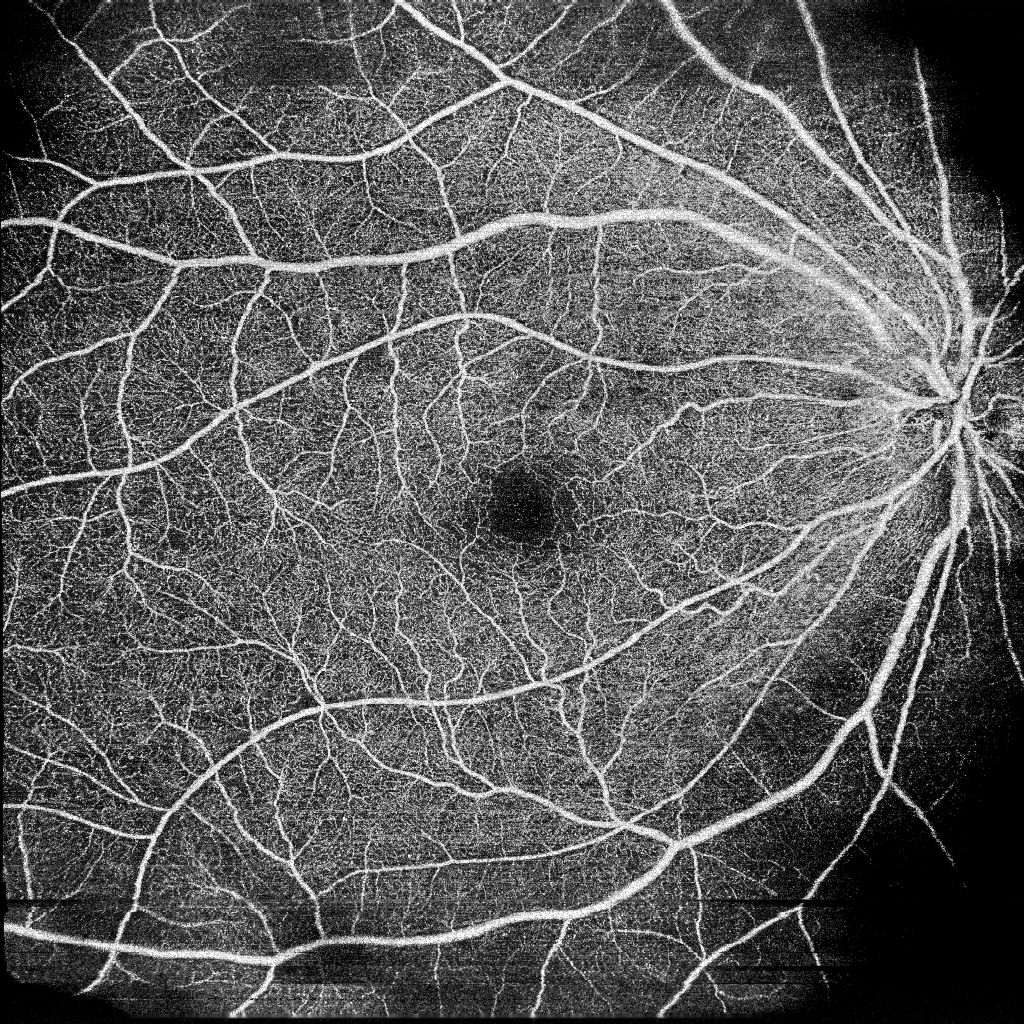
\includegraphics[scale=0.2]{gambar/exampleimage.png}
  % Keterangan gambar yang diinputkan
  \caption{Contoh Data Citra Retina}
  % Label referensi dari gambar yang diinputkan
  \label{fig:citraRetina}
\end{figure}

\textbf{Peralatan}

Dalam penelitian ini, penulis menggunakan komputer dengan sistem operasi Windows 11 dengan spesifikasi sebagai berikut:
\begin{itemize}
  \item Processor: Intel Core i5 12400F
  \item RAM: 16GB 3200MHz
  \item GPU: NVIDIA GeForce RTX 3060 Ti
  \subitem CUDA Cores: 4864
  \subitem Memory Config: 8 GB GDDR6
\end{itemize}

\emph{Software} yang digunakan dalam penelitian ini adalah sebagai berikut:
\begin{itemize}
  \item Jupyter Notebook
  \item Visual Studio Code
\end{itemize}

\section{Metode yang digunakan}


% Contoh input gambar dengan format *.jpg
\begin{figure} [H] \centering
  % Nama dari file gambar yang diinputkan
  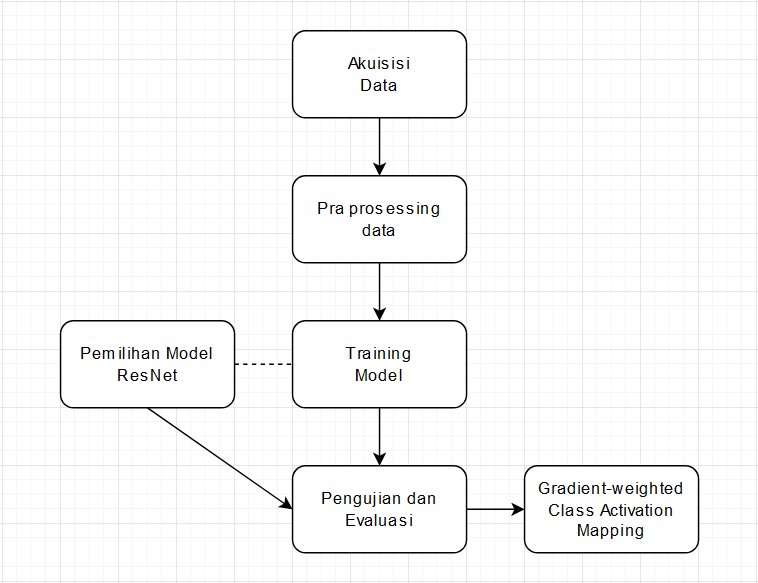
\includegraphics[scale=0.5]{gambar/diagramMethod.png}
  % Keterangan gambar yang diinputkan
  \caption{Diagram blok metodologi}
  % Label referensi dari gambar yang diinputkan
  \label{fig:diagramMethod}
\end{figure}

% Contoh penggunaan referensi dari gambar yang diinputkan
\subsection{Akuisisi Data}
Data yang digunakan dalam penelitian ini adalah data yang diperoleh dari Diabetic Retinopathy Analisis Grand challenge \parencite{drac_challenge_2023_10280359}. Data yang digunakan adalah data citra retina yang sudah diberi label berupa tingkat keparahan penyakit retinopati diabetik yang sebelumnya sudah melalui proses image assesment sehingga sudah siap digunakan untuk training model. Dataset ini berisikan 611 citra OCT-A yang telah diberi label. Dataset ini juga berisikan 386 citra OCT-A yang tidak berlabel untuk dijadikan testing dataset.

\subsection{Pra-pemrosesan Data}
Pra-pemrosesan data dilakukan untuk mempersiapkan data sebelum dilakukan proses pelatihan model. Pra-pemrosesan data yang dilakukan adalah konversi citra retina dari format .jpeg menjadi .png. Hal ini dilakukan karena format .png memiliki ukuran yang lebih kecil dibandingkan dengan format .jpeg. Selain itu, format .png juga tidak mengurangi kualitas citra retina. Pra-pemrosesan data juga dilakukan untuk membagi data menjadi data latih dan data uji. Data latih digunakan untuk melatih model sedangkan data uji digunakan untuk menguji model.

\subsection{ Model ResNet}
Model ResNet yang akan digunakan untuk dibandingkan dalam penelitian ini adalah model pre-trained resnet-18, resnet-34, resnet-50, resnet-101, dan resnet-152. Performa model-model tersebut akan dibandingkan dengan melihat nilai akurasi, \emph{loss}, dan \emph{val\_loss}.

\subsection{Pelatihan Model}
Pelatihan model dilakukan dengan menggunakan metode \emph{transfer learning}. Metode \emph{transfer learning} dilakukan dengan menggunakan model ResNet yang sudah dipilih dan sudah dilatih dengan dataset ImageNet.

\subsection{Pengujian dan Evaluasi}
Pengujian dan evaluasi dilakukan dengan menggunakan data uji. Pengujian dan evaluasi dilakukan dengan melihat nilai akurasi, \emph{loss}, dan \emph{val\_loss}. Selain itu, pengujian dan evaluasi juga dilakukan dengan melihat \emph{confusion matrix} dari model yang sudah dilatih, untuk dilihat nilai presisi, recall, dan F1 pada setiap kelasnya, untuk melihat performa model dalam memprediksi tingkat keparahan penyakit retinopati diabetik.

\subsection{Gradient-weighted Class Activation Mapping}
Grad-CAM digunakan untuk mengetahui faktor-faktor yang mempengaruhi model dalam memprediksi tingkat keparahan penyakit retinopati diabetik. Grad-CAM bekerja dengan menghitung gradien output model terhadap input, dan kemudian menggunakan gradien tersebut untuk memprediksi area input yang paling berkontribusi pada output model.

\cleardoublepage

% Konten lainnya
\chapter{HASIL}

\section{Hasil yang Diharapkan}

Penelitian ini diharapkan untuk:
\begin{enumerate}
    \item Mengembangkan model ResNet untuk deteksi dan klasifikasi DR.
    \item Mengidentifikasi fitur-fitur utama yang berkontribusi pada pengambilan keputusan model, yang berpotensi meningkatkan kemampuan interpretasi dan kepercayaan.
    %\item Mendemonstrasikan potensi pendekatan berbasis ResNet untuk implementasi yang lebih luas dalam pengaturan klinis.
\end{enumerate}

\section{Hasil Pendahuluan}

Sampai saat ini, kami telah \lipsum[16]

\cleardoublepage

% Konten jadwal penelitian
\chapter{JADWAL PENELITIAN}

% Ubah tabel berikut sesuai dengan isi dari rencana kerja
\newcommand{\w}{}
\newcommand{\G}{\cellcolor{gray}}
\begin{table}[H]
  \captionof{table}{Tabel timeline}
  \label{tbl:timeline}
  \begin{tabular}{|p{3.5cm}|c|c|c|c|c|c|c|c|c|c|c|c|c|c|c|c|}

    \hline
    \multirow{2}{*}{Kegiatan}          & \multicolumn{16}{|c|}{Minggu}                                                                       \\
    \cline{2-17}                       &
    1                                  & 2                             & 3  & 4  & 5  & 6  & 7  & 8  & 9  & 10 & 11 & 12 & 13 & 14 & 15 & 16 \\
    \hline

    % Gunakan \G untuk mengisi sel dan \w untuk mengosongkan sel
    Pengambilan data                   &
    \G                                 & \G                            & \w & \w & \w & \w & \w & \w & \w & \w & \w & \w & \w & \w & \w & \w \\
    \hline

    Pengolahan dan training data citra &
    \w                                 & \w                            & \G & \G & \G & \G & \G & \G & \w & \w & \w & \w & \w & \w & \w & \w \\
    \hline

    Pembuatan model prediksi           &
    \w                                 & \w                            & \w & \w & \w & \w & \w & \w & \G & \G & \G & \G & \w & \w & \w & \w \\
    \hline

    Analisa dan Evaluasi model         &
    \w                                 & \w                            & \w & \w & \w & \w & \w & \w & \w & \w & \w & \G & \G & \G & \G & \w \\
    \hline

    Penyusunan laporan                 &
    \w                                 & \w                            & \w & \w & \w & \w & \w & \w & \w & \w & \G & \G & \G & \G & \G & \G \\
    \hline
  \end{tabular}
\end{table}

Pada Tabel \ref{tbl:timeline} dapat dilihat bahwa penelitian ini akan dilakukan selama 16 minggu. Tahap pertama adalah pengambilan data yang akan dilakukan pada minggu pertama. Tahap kedua adalah pengolahan dan training data citra yang akan dilakukan pada minggu ke-3 sampai minggu ke-6. Tahap ketiga adalah pembuatan model prediksi yang akan dilakukan pada minggu ke-9 sampai minggu ke-12. Tahap keempat adalah analisa dan evaluasi model yang akan dilakukan pada minggu ke-13 sampai minggu ke-16. Tahap kelima adalah penyusunan laporan yang akan dilakukan pada minggu ke-13 sampai minggu ke-16.

\cleardoublepage


% Daftar pustaka
\chapter*{DAFTAR PUSTAKA}
\addcontentsline{toc}{chapter}{DAFTAR PUSTAKA}
\renewcommand\refname{}
\vspace{2ex}
\renewcommand{\bibname}{}
\begingroup
\def\chapter*#1{}
\printbibliography
\endgroup


\end{document}
